\chapter{Related Work}
\label{chapter:ch2}

In Chapter~\ref{chapter:ch2}, an in-depth exploration of the relevant literature. We begin by exploring the concept of Transformer Attention, a fundamental mechanism extensively utilized in various vision and language models (Sec.~\ref{transformer}). We also explore its variants, such as the Vision Transformer (Sec.~\ref{vit}) and the Language Transformer (Sec.~\ref{language transformer}), which have revolutionized the field of deep learning by effectively capturing complex relationships within visual and textual data. Furthermore, we provide an in-depth analysis of the recent advancements in vision-language pre-training techniques (Sec.~\ref{vlp}). These methodologies involve extensive pre-training on large-scale datasets incorporating both visual and textual data, aiming to acquire highly robust multimodal representations. Next, a comprehensive exploration is conducted on the concept of Visual Question Answering (Sec.~\ref{vqa}), which involves answering questions about an image using both visual and textual information. Finally, we then narrow our focus to Medical Visual Question Answering (Sec.~\ref{medvqa}), a specialized domain where VQA techniques are applied to medical images and associated medical knowledge. By conducting a thorough analysis of the previous literature, this chapter offers a comprehensive insight into the challenges and recent advancements within the domain of vision-language pre-training in the medical domain, thus laying the foundation for the formulation of our proposed approach.

% In Chapter~\ref{chapter:ch2}, an in-depth exploration of the relevant literature. We begin by exploring the concept of Visual Question Answering (Sec.~\ref{vqa}), which involves answering questions about an image using both visual and textual information. We then narrow our focus to Medical Visual Question Answering (Sec.~\ref{medvqa}), a specialized domain where VQA techniques are applied to medical images and associated medical knowledge. Next, a comprehensive exploration is conducted on Transformer Attention, a fundamental mechanism extensively utilized in various vision and language models (Sec.~\ref{transformer}). We also explore its variants, such as the Vision Transformer (Sec.~\ref{vit}) and the Language Transformer (Sec.~\ref{language transformer}), which have revolutionized the field of deep learning by effectively capturing complex relationships within visual and textual data. Furthermore, we provide an in-depth analysis of the recent advancements in vision-language pre-training techniques (Sec.~\ref{vlp}). These methodologies involve extensive pre-training on large-scale datasets incorporating both visual and textual data, aiming to acquire highly robust multimodal representations. Finally, we explore the advancements made in leveraging pre-training techniques specifically for medical images and associated text (Sec.~\ref{medvlp}), enabling the model to acquire specialized medical knowledge and improve performance in medical vision-language tasks. By conducting a thorough analysis of the previous literature, this chapter offers a comprehensive insight into the challenges and recent advancements within the domain of vision-language pre-training in the medical domain, thus laying the foundation for the formulation of our proposed approach.

\section{Transformer Attention}
\label{transformer}
The transformer \cite{vaswani2017attention} is a revolutionary deep learning architecture that has had a profound impact on various domains, including natural language processing and computer vision. Unlike traditional sequential models, such as recurrent neural networks (RNNs) \cite{rumelhart1985learning}, transformers process entire input sequences in parallel, making them highly efficient for capturing long-range dependencies. As shown in Figure~\ref{fig:transformer}, the transformer model consists of an encoder and a decoder, with each component containing multiple layers of self-attention and feed-forward neural networks. A fundamental element of the transformer is its attention mechanism, which enables the model to assign varying degrees of importance to different components within the input sequence, facilitating more accurate predictions.

The attention mechanism operates from the perspective of queries $Q$, keys $K$, and values $V$; see formula~\ref{eq:attention}. In this mechanism, queries represent the current input element that needs to attend to other elements in the sequence. Keys and values correspond to the other elements in the sequence. The attention mechanism computes the similarity between the query and each key using a dot product or a learned similarity function. These similarities determine the relevance or importance of each key with respect to the query. Then, the attention scores are normalized to obtain attention weights, which indicate the relative importance of each value. The final step involves calculating a weighted sum of the values, where the weights are determined by the attention weights; see Figure~\ref{fig:attention} (a). This process allows the model to give more attention to relevant parts of the input sequence while suppressing irrelevant or noisy information. 

\begin{equation}\label{eq:attention}
    Attention(Q, K, V) = softmax(\frac{QK^T} {\sqrt{d_k}})V 
\end{equation}


Multi-head attention is an essential component of the transformer architecture that further enhances its modeling capabilities. As shown in Figure~\ref{fig:attention} (b), the attention mechanism is applied multiple times in parallel, with each attention head learning different aspects of the input sequence. Each attention head operates on its own learned linear projections of the input, allowing for the simultaneous extraction of different features and representations. After computing attention independently for each head, the outputs are concatenated and linearly transformed to generate the final attention output. Using multiple attention heads allows the model to capture different patterns and relationships in the data at different levels of detail

\begin{figure}
\centering
\scalebox{0.7}{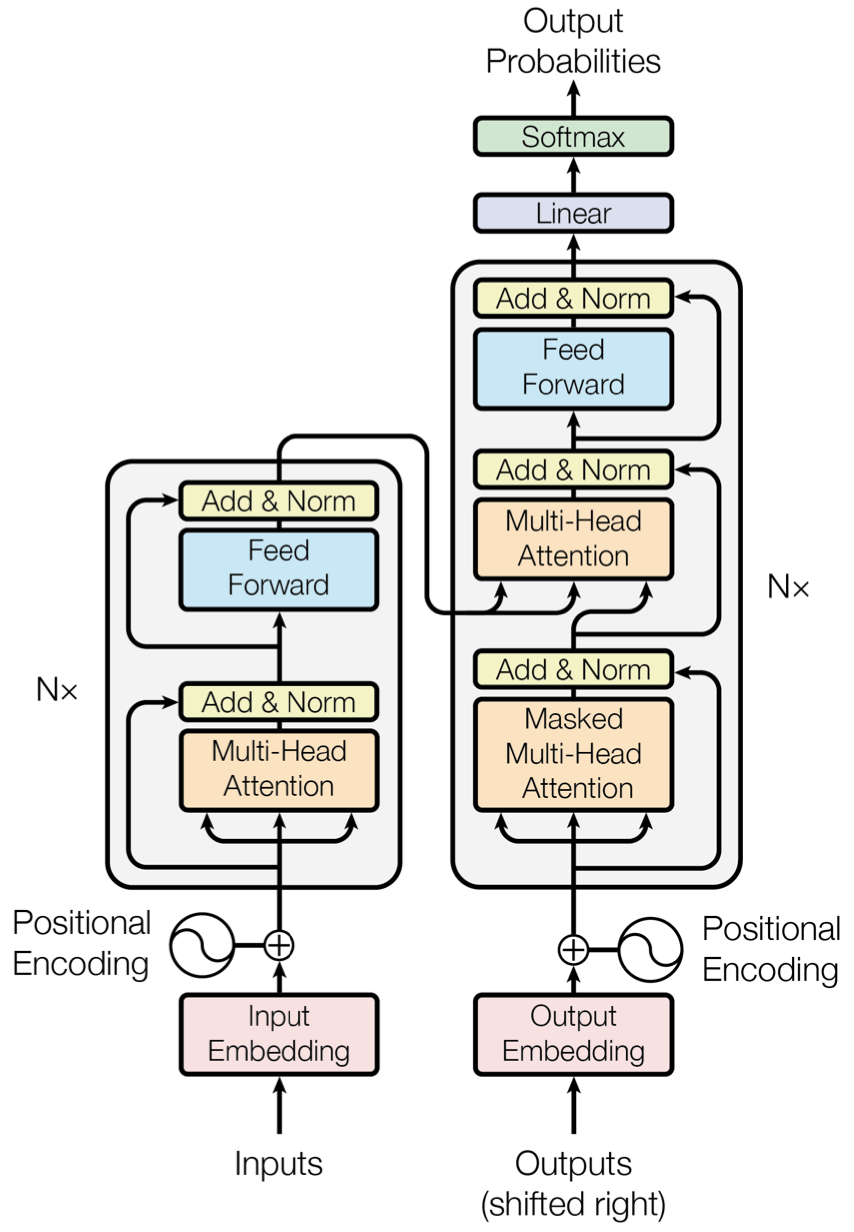
\includegraphics[width=1\textwidth]{Chapter_2/transformer.png}}
\caption{Transformer architecture \cite{vaswani2017attention}}
\label{fig:transformer}
\end{figure}

\begin{figure}
\centering
\scalebox{0.9}{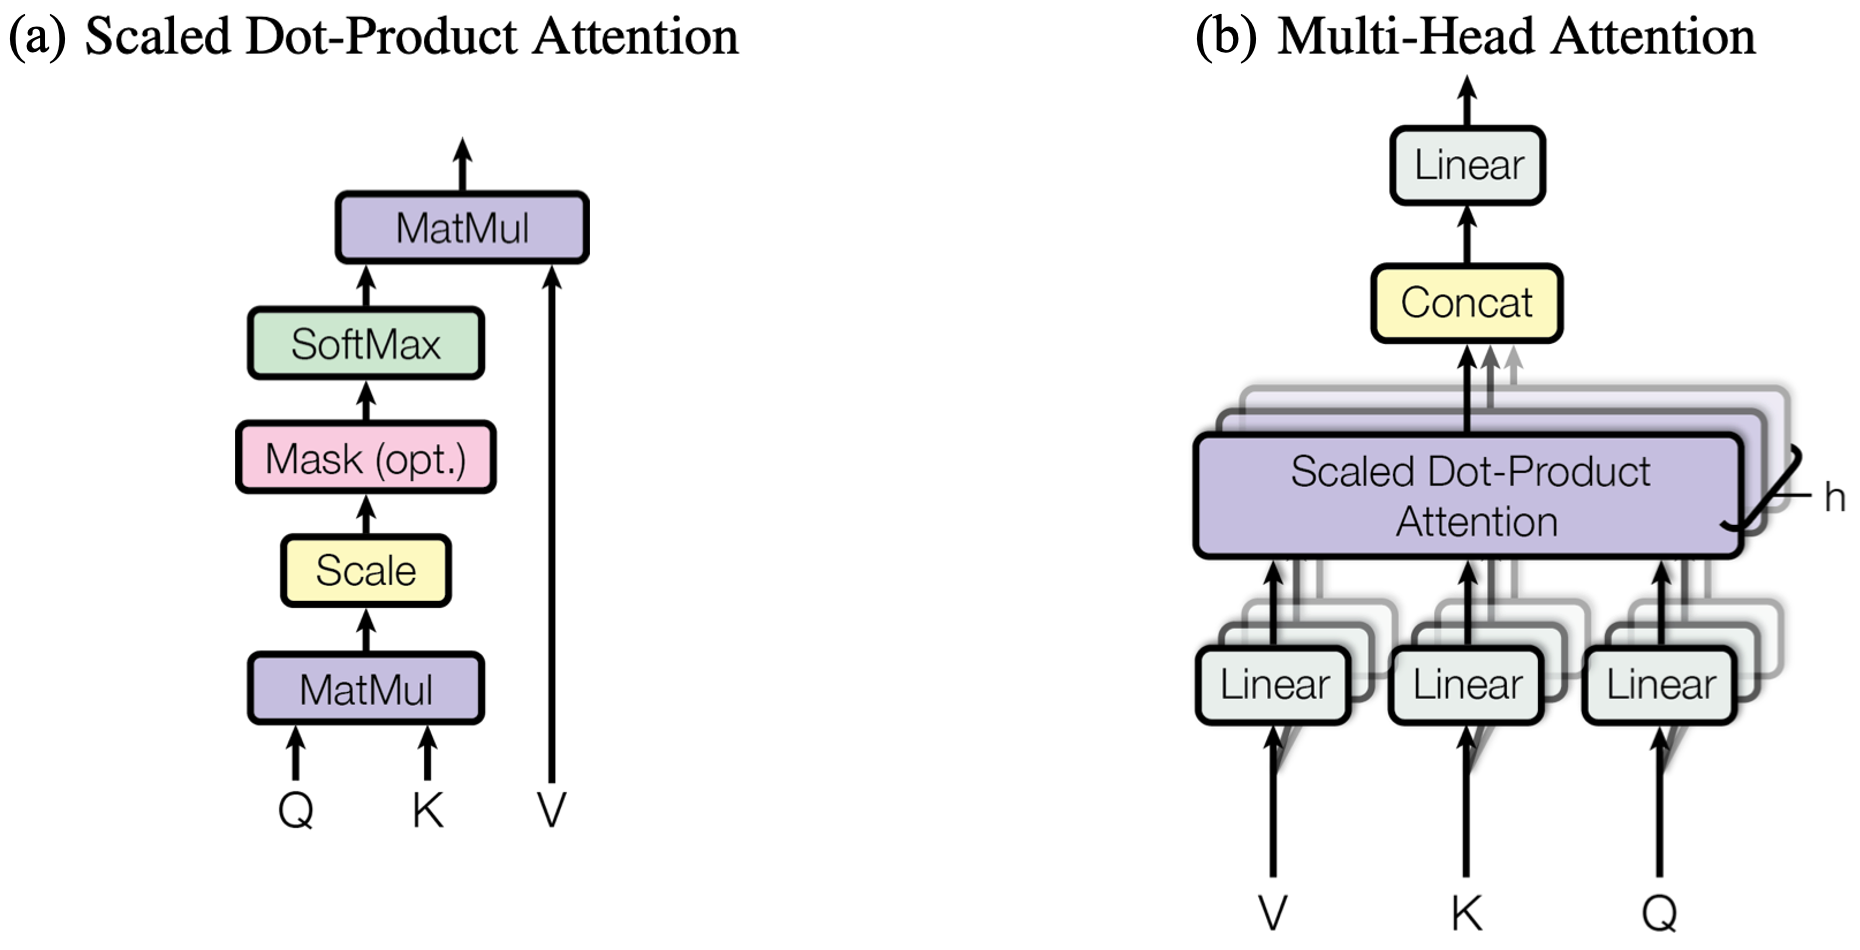
\includegraphics[width=1\textwidth]{Chapter_2/attention.png}}
\caption{Attention mechanisms \cite{vaswani2017attention}: (a) Scaled dot-product attention, (b) Multi-head attention}
\label{fig:attention}
\end{figure}
 


\subsection{Vision Transformer}
\label{vit}
The Vision Transformer (ViT) \cite{dosovitskiy2020vit} is a popular architecture for visual tasks that adapts the transformer model from natural language processing. It divides the input image into fixed-size patches and maps them to token embeddings, which are then processed by the transformer encoder to capture global relationships among the patches. This allows the ViT to learn representations for various vision tasks. The model efficiently converts the input image with dimensions $(C, H, W)$ into an image representation with dimensions $(C, H/16, W/16)$, where $C$ is the number of channels, $H$ is the height of the image, and $W$ is the width of the image.

Swin Transformer \cite{Liu_2021_ICCV} is one of the variants that introduces hierarchical representations by stacking multiple stages of transformers. It divides the image into non-overlapping patches at the initial stage and applies transformers at different scales, capturing both local and global information. Swin Transformer leverages shifted windows and window partitioning to efficiently model long-range dependencies while reducing computational complexity. This variant has shown improved performance and scalability, making it an appealing choice for visual recognition tasks, especially when dealing with high-resolution images or large-scale datasets.

\subsection{Language Transformer}
\label{language transformer}
The Language Transformer is a powerful architecture for natural language processing tasks. It is based on the transformer attention model. The language transformer can be classified into two architectural categories: encoder-only and encoder-decoder. 

An example of the encoder-only architecture is the BERT model \cite{devlin-etal-2019-bert}. BERT employs a masked language modeling objective, where it randomly masks certain tokens in the input and predicts them based on the surrounding context. This allows BERT to learn deep bidirectional representations that capture both the left and right context of each token.

In contrast, The encoder-decoder architecture shares the same foundational structure as the architecture described in \cite{vaswani2017attention}. This setup is commonly used in generative models, such as the GPT model \cite{brown2020language}. The encoder-decoder architecture is widely used for tasks like machine translation and text generation. The encoder processes the input sequence, while the decoder generates the output sequence autoregressively, attending to the encoder's representations to produce contextually informed predictions at each step.


\section{Vision and Language Pre-Training}
\label{vlp}
Vision and language pre-training techniques \cite{Dou_2022_CVPR, li2020oscar, li2022blip, li2021align, tan2019lxmert, lu2019vilbert} involve self-supervised learning using a combination of image and caption data. This approach has shown promising results in various vision-language downstream tasks, such as visual question answering. As illustrated in Figure~\ref{fig:pretrainFinetune}, the Vision and Language pre-training consists of two phases: the pre-training phase and the fine-tuning phase. During the pre-training process, a model is trained on a large corpus of image-caption pairs without relying on explicit annotations. Subsequently, the model is fine-tuned on various downstream tasks, such as visual question answering. This allows the model to learn meaningful representations that capture the relationship between visual and textual information.

In vision and language pre-training, two common objectives are employed: masked language modeling (MLM) and image-text matching (ITM).

Masked language modeling is a form of self-supervised learning objective where a portion of the input text is randomly masked, and the model is tasked with predicting the masked words based on the context provided by the surrounding words and the corresponding image; see Figure~\ref{fig:mlm}. Typically, two fully connected layers (referred to as the Masked Language Modeling Head) are appended to the model. This component allows the model to predict masked tokens within the input text, improving its ability to learn contextual representations and capture vision-language patterns.

\begin{figure}
\centering
\scalebox{0.7}{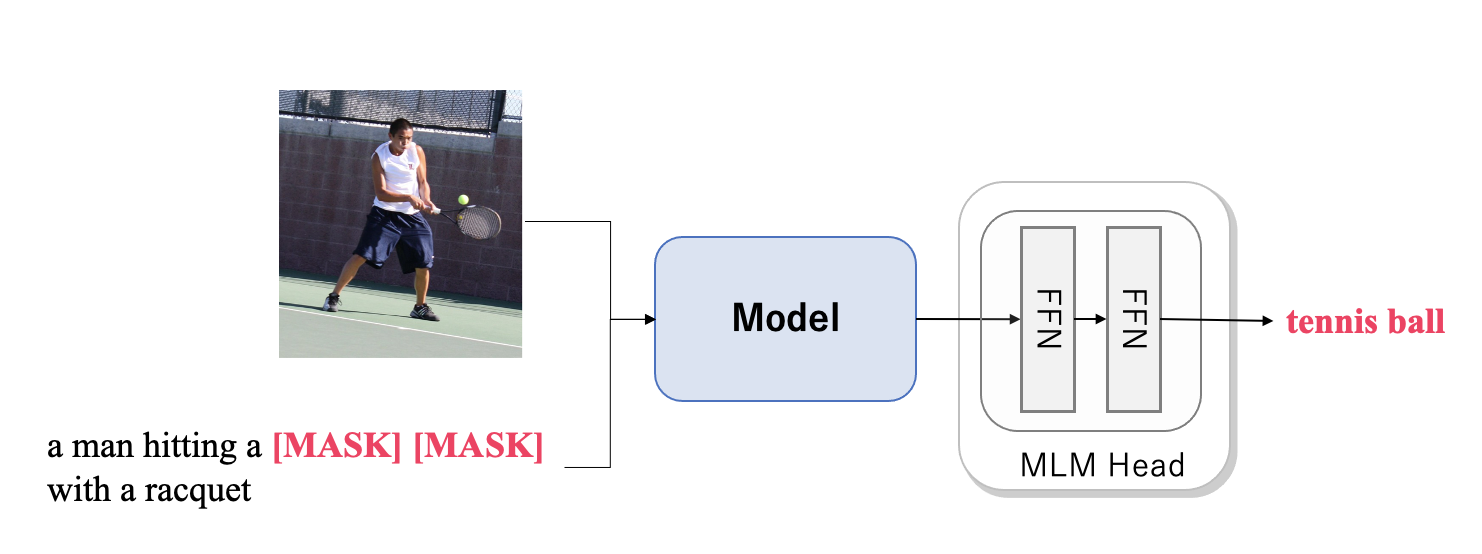
\includegraphics[width=1\textwidth]{Chapter_2/MLM.png}}
\caption{Masked language modeling \cite{Dou_2022_CVPR}}
\label{fig:mlm}
\end{figure}

Image-text matching aims to align the image and text representations by training the model to determine whether a given image and its corresponding caption are a correct match; see Figure~\ref{fig:itm}. The model is extended with an image-text matching head, which incorporates two fully connected layers as depicted in Figure~\ref{fig:itmhead}. By optimizing this objective, the model develops the ability to relate visual and textual information effectively. 

\begin{figure}
\centering
\scalebox{0.7}{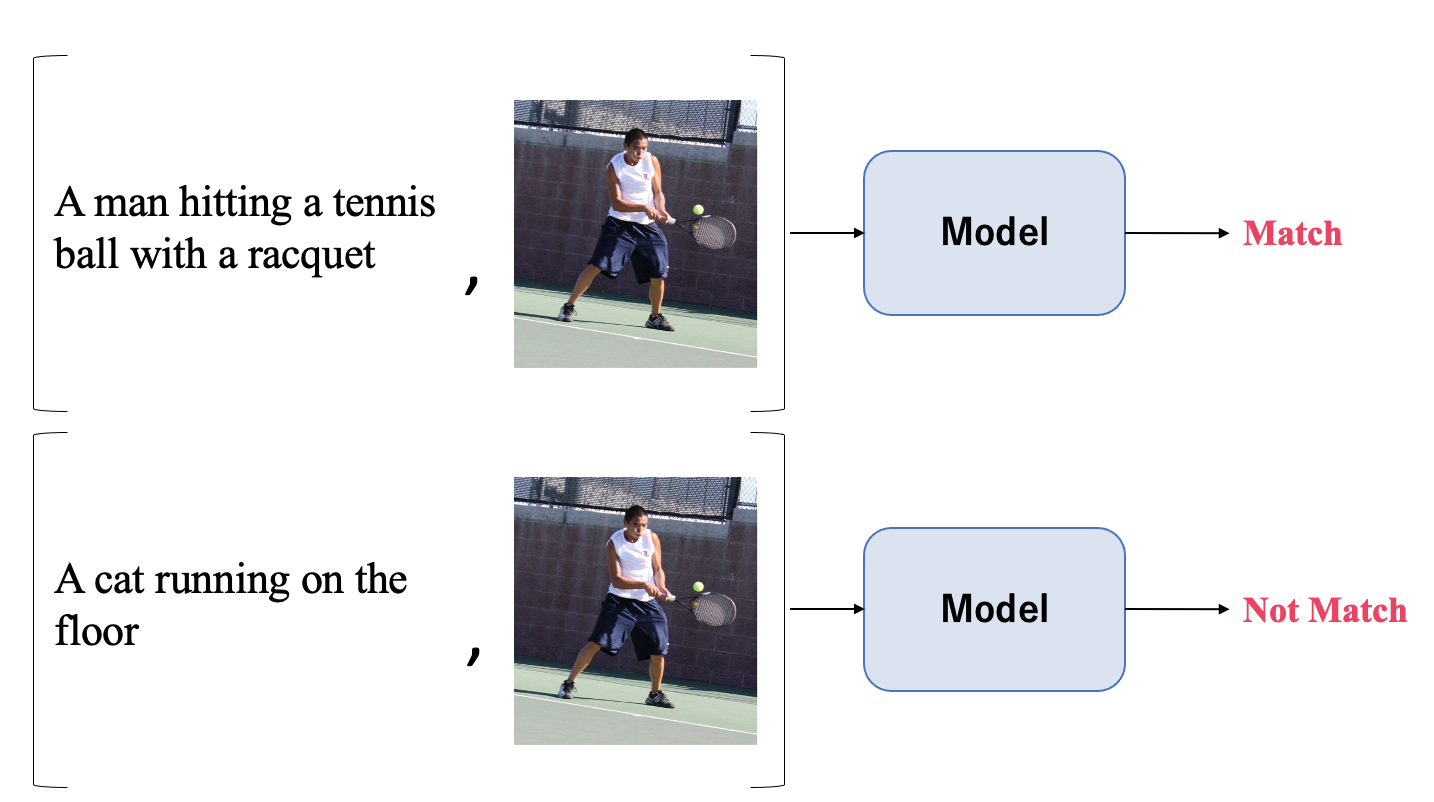
\includegraphics[width=1\textwidth]{Chapter_2/ITM.png}}
\caption{Image-text matching \cite{Dou_2022_CVPR} involves determining whether an image and its corresponding caption are a match or not. The top image represents a positive pair, indicating a matching image and caption. On the other hand, the bottom image represents a negative pair, indicating a non-matching image and caption.}
\label{fig:itm}
\end{figure}

\begin{figure}
\centering
\scalebox{0.7}{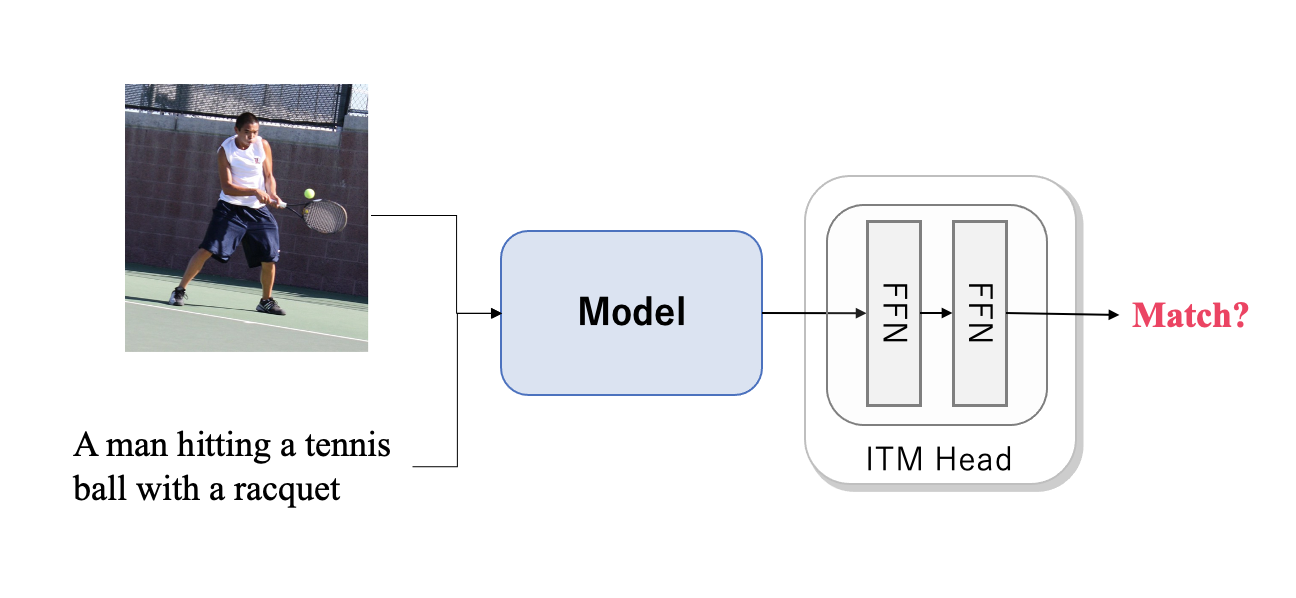
\includegraphics[width=1\textwidth]{Chapter_2/chap2_itmhead.png}}
\caption{
The image-text matching head \cite{Dou_2022_CVPR} consists of two fully connected layers in its architecture.}
\label{fig:itmhead}
\end{figure}

Through self-supervised learning with MLM and ITM, the vision and language pre-training technique enables the model to acquire a rich understanding between visual and textual modalities. This knowledge can then be leveraged in downstream tasks, where the model can generalize well and provide accurate predictions and answers based on both visual and textual inputs.


\section{Visual Question Answering}
\label{vqa}
Visual Question Answering (VQA) \cite{VQA, balanced_binary_vqa, balanced_vqa_v2} is a task that aims to answer questions based on the content of an image. As shown in Figure~\ref{fig:vqa}, it involves providing a model with both an image and a corresponding question as input and expecting the model to generate the appropriate answer. VQA combines computer vision and natural language processing techniques to bridge the gap between visual information and textual understanding. 

\begin{figure}[t]
\begin{center}
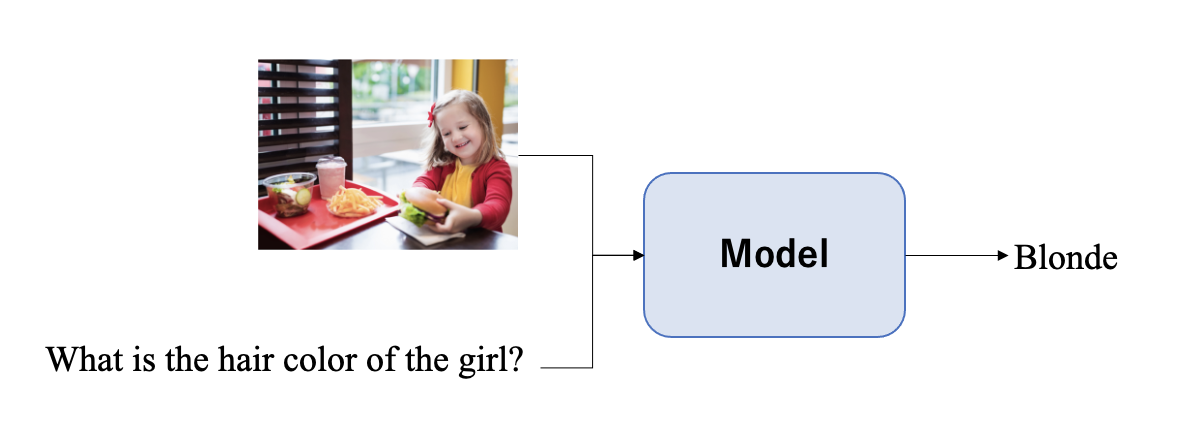
\includegraphics[width=1.0\linewidth]{Chapter_2/chap2_vqa.png}
\end{center}
   \caption{Visual question answering \cite{liu2022dpt} is a task in which a model takes images and corresponding questions as input and generates accurate answers as output.
}
\label{fig:vqa}
\end{figure}

\section{Medical Visual Question Answering}
\label{medvqa}
Medical Visual Question Answering (Medical VQA) \cite{liu2021slake, DBLP:journals/corr/abs-2003-10286, lau2018dataset, ben2019vqa} is a specialized task that applies the techniques of Visual Question Answering to the medical domain. It involves answering questions related to medical images or healthcare scenarios using both visual and textual information. There are two types of previous work in this field: models that utilize pre-training \cite{chen2022align, chen2023towards, moon2022multi, chen2022multi, khare2021mmbert} and models that do not rely on pre-training \cite{liu2021slake, nguyen2019overcoming, do2021multiple, gong2022vqamix, zhang2022type}. Generally, the approaches that employ pre-training models tend to exhibit state-of-the-art performance in this field. However, this thesis aims to illustrate that the direct application of vision-language pre-training techniques in the medical domain may not yield optimal outcomes. Instead, we propose novel techniques to enhance the performance applicability of the task.



% \section{Medical Vision and Language Pre-Training}
% \label{medvlp}
% Medical vision and language pre-training techniques \cite{chen2022align, chen2023towards, moon2022multi, chen2022multi, khare2021mmbert} extend the concept of vision-language pre-training to the medical domain, showcasing promising performance in various healthcare applications, such as generating accurate and contextually relevant medical reports or diagnoses. By conducting pre-training specifically on medical data, these techniques enable models to develop a deeper understanding of medical images and their corresponding textual information. 

% Furthermore, medical vision and language pre-training has demonstrated its efficacy in medical visual question answering (VQA), allowing models to comprehend medical images and answer questions related to them. This capability can be highly beneficial in assisting healthcare professionals by automating certain tasks and providing reliable and timely information. 

% With the state-of-the-art performance achieved in medical downstream tasks, medical vision and language pre-training techniques have the potential to revolutionize the field of healthcare. By leveraging their understanding of medical images and textual data, these models can support medical professionals in making accurate diagnoses, conducting research, and providing personalized patient care. 
% \textcolor{red}{however, they are two problems if we simply apply medical in vlp, and this thesis try to solve this problem.}